% !TEX root = 15cvpr.tex

\section{The Proposed Model}

We formulate the semantic segmentation problem as an Conditional Random Field (CRF) over image superpixels incorporating various contextual relations, for instance, the associations between high-level semantic concepts and low-level visual appearance, and the label consistency between image-level and pixel-level, to advance segmentation performance, even in noisy real-world settings. Moreover, the connections among semantic labels, which are captured by two aspects, inter-label co-occurrence statistics as well as discriminative regions overlap of concepts pairs, are integrated to determine latent associations for annotation noise reduction.

More formally, suppose we have a set of weakly labeled images $\mathcal{I}=\{I_k\}_{k=1}^N$, where $N$ donates the total number of training images. Each image $I$ is associated with a vector of the $L$ binary variables $\boldsymbol{y} = (y_1,...,y_L)^{\rm T}$, \ie $y_i \in \{0,1\}$, where $y_i=1$ indicates that the $i$-th category is present in this image, and $0$ otherwise.

We adopt a superpixel representation of each image $I$, where the superpixels are generated from multi-scale segmentation algorithm. Then we associate every superpixel $x_p$ ($p \in \mathcal{V}$) with a random variable $h_p \in \mathcal{C}$ to represent its semantic category. Here, $\mathcal{V} = \{1,...,M\}$ is a set of all the superpixels in image $I$ and $M$ indicates the total number of superpixels. Besides, $\mathcal{C} = \{1,...,L\}$ denotes the set of predefined labels.

Our goal is to find the accurate semantic label for each pixel in an image and the adjacent pixels sharing the same semantic label are fused as the whole one. To tackle this problem, we build a Conditional Random Field (CRF) on the image-level label variables $\boldsymbol{y}$ and the superpixel-level label variables $\boldsymbol{h}$. We connect each superpixel variables to its neighbors to encode a local smoothness constraint. Specifically, let $\mathcal{E}$ donate the neighborhood system among the superpixels, we define an energy function $E$ with five types of potential as follows:
\begin{equation}
    \label{eq:energyfunction}
    \begin{aligned}
        E(\boldsymbol{y},\boldsymbol{h},I&) = \sum_{i=1}^L{\psi_{G}(y_i,I)}
                            + \sum_{1 \le i,j \le L} {\psi_{R}(y_i,y_j)}\\ &+ \sum_{p \in \mathcal{V}}{\psi_{L}(h_p,x_p)}+ \sum_{(p,q) \in \mathcal{E}}{\psi_{S}(h_p,h_q)}\\ &+ \psi_{C}(\boldsymbol{y},\boldsymbol{h})
    \end{aligned}
\end{equation}
where $\psi_G$ and $\psi_{L}$ encode the unary potential of global and regional constraints respectively, $\psi_R$ impose label correlation and co-occurrence, $\psi_S$ are the spatial context constraints for each superpixel, and $\psi_C$ ensure the consistency between global and regional labels.  The posterior distribution $P(\boldsymbol{y},\boldsymbol{h}|I)$ of the CRF can be written as $P(\boldsymbol{y},\boldsymbol{h}|I) = \frac{1}{Z(I)}\exp{\{-E(\boldsymbol{y},\boldsymbol{h},I)\}}$, where $Z(I)$ is the normalizing constant. Thus, the most probable labeling configuration $\boldsymbol{y}^{\star},\boldsymbol{h}^{\star}$ of the random field can be defined as  $\boldsymbol{y}^{\star},\boldsymbol{h}^{\star} = \arg \min_{\boldsymbol{y},\boldsymbol{h}} E(\boldsymbol{y},\boldsymbol{h},I)$. The details of each potential will be described in the following sections, and a graphical representation of the energy function is shown in Figure \ref{fig:graphmodel}

\if
 We utilize a label classifier which leverages convolutional Neural Network(CNN) for noisy label refinement.\cite{agrawal2014analyzing} shows that fine-tuning a discriminatingly pre-trained network is very effective in terms of task performance. Unfortunately, the appearance model cannot be trained or fine-tuned directly due to the fact that the assignment of superpixels to semantic labels is unknown, even at training time.
\fi

\begin{figure}[t]
    \begin{center}
        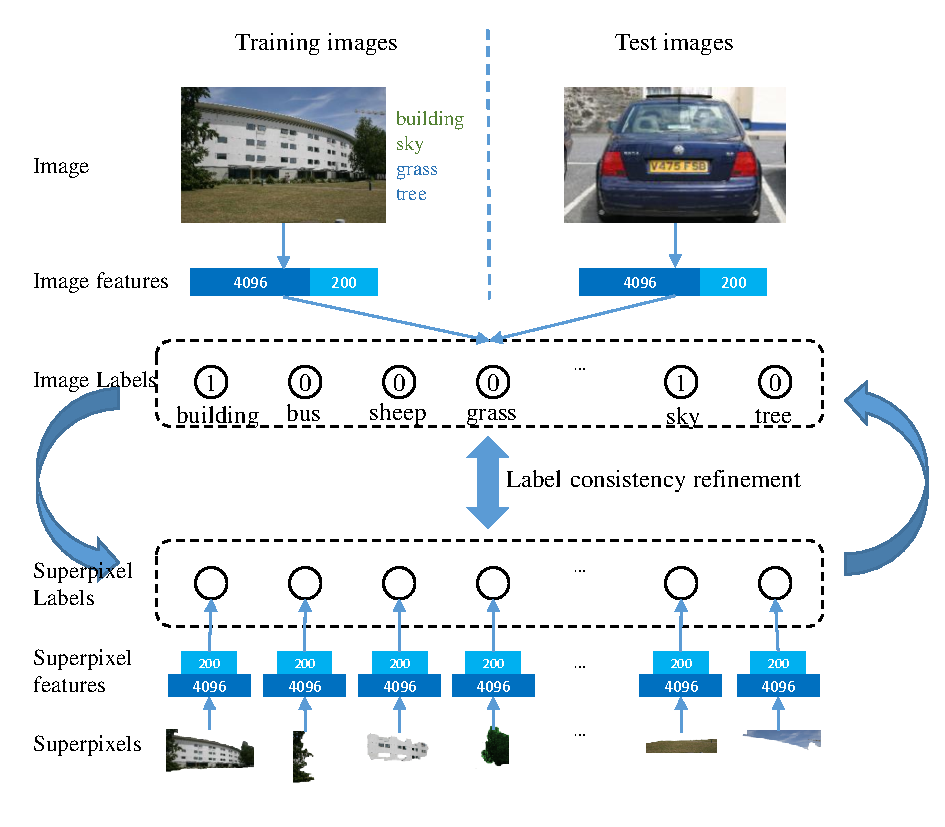
\includegraphics[width=1\linewidth]{fig_framework.pdf}
    \end{center}
    \caption{Example of a short caption, which should be centered.}
    \label{fig:framework}
\end{figure}

\subsection{Unary Potential}
\textbf{Image-Level Potential}
We model input image by two aspects: On the one hand, we utilize convolutional neural network (CNN) to represent the appearance model of each image, especially the first fully-connected layer containing 4096 neurons of a 19-layers model \cite{simonyan2014very}. On the other hand, for topic model, we model the CNN representation as a finite mixture of latent semantic concepts by probabilistic latent semantic analysis (pLSA) \cite{sivic2005discovering}, which can recover visual models of semantic labels in a completely unsupervised manner.
\if
Probabilistic latent semantic analysis (pLSA) is a probabilistic model that is well suited to weakly supervision. Each image has its own mixing proportions whereas the topics are shared by all images. In document analysis, the pLSA usually takes the histogram of occurrence frequency on words as input. 
\fi
Similar to \cite{wang2014weakly}, we regard fully-connected layer as input considering each neuron as a visual word $w_i$ and each image as a document $d_j$, then the occurrence frequency of image on $w_i$ is the i-th dimension of $d_j$. In addition, there is a hidden semantic topic variable $t_k$ associated with all the visual words. We treat each topic $t_k$ as a latent category in a semantic label. The pLSA optimizes the joint probability $P(w_i,d_j,t_k)$. Marginalizing over the latent category $t_k$ determines the conditional probability $P(w_i|t_k)$:
\begin{equation}
  P(w_i|d_j) = \sum_{k=1}^K{P(t_k|d_j)P(w_i|t_k)}
\end{equation}
where $P(t_k|d_j)$ is the probability of topic $t_k$ occurring in image $j$. Formally we formulate image-level feature as $I$ by concatenating the appearance feature $d_j$ and topic distribution $P(\boldsymbol{t}|d_j)$, and define the image-level label presence potential $\psi_{G}$ as follows:
\begin{equation}
    \psi_{G}(y_i,I) = -\log f_{i}(I)
    \label{eq:global}
\end{equation}
where $f_{i}(I)$ is the classifier score function associated with label $i$.

\textbf{Superpixel-Level Potential}
Similar with image-level potential, we both consider the appearance model and topic model in order to narrow down the gap between low-level feature space and high-level semantic space, in the meantime, to reduce the influence of inaccurate image-level labels. Formally, we encode the unary potential of regions as follows:
\begin{equation}
    \begin{aligned}
        \psi_{L}(h_p,x_p) = &- \log \big\{ w_1\phi_a(h_p,a_p,\theta_a) \\
        &+ w_2\phi_t(h_p,t_p,\theta_t) \big\}
    \end{aligned}
    \label{eq:local}
\end{equation}
where $a_p, t_p$ are the appearance and topic feature vectors extracted from the superpixels, $\theta_a, \theta_t$ donate the parameters with respect to appearance model and topic model, $\{w_i\}|_{i=1}^2$ are the weighting coefficients for the unary terms. We define the appearance model $\phi_a(h_p,a_p,\theta_a) = f_{h_p}(a_p,\theta_a)$ and topic model $\phi_t(h_p,t_p,\theta_t) = g_{h_p}(t_p,\theta_t)$ measuring how well the local appearance $a_p$ and topic $t_p$ matches the semantic label $h_p$.

\subsection{Pairwise Potential}

\textbf{Label Correlation}
We model inter-label co-occurrence by constructing inter-label correlation matrix which characterizing the interaction between semantic concepts and helps to model the relationship among feature space of superpixels. Due to the unknown semantic annotation of superpixels, learning these latent information is an unsupervised learning problem. Moreover, the context contain some useful latent information which can be learned for semantic label noise reduction.

Here we consider two aspects to construct inter-label matrix, on the one hand, we construct co-occurrence matrix $Cooc$ to capture the inter-label correlation. $Cooc$ is an $L \times L$ symmetric matrix and its entry $Cooc(i,j)$, measuring the co-occurrence of concepts pair $(i,j)$ based on statistics, can be defined as follows:
\begin{equation}
    Cooc(i,j) = 1-(1-P(i|j))(1-P(j|i))
\end{equation}

On the other hand, we determine the inter-label correlation via \textcolor{red}{discriminative regions overlap of concepts pair}. The discriminative region of concept indicates the most informative sub-windows of each image within a multi-class classification framework. The basic idea is to analyze the variation of classification score when artificially blackout different regions of the image. We observe that blackout a discriminative sub-window causes a massive confusion for one-vs-one classifier, especially in cluster condition. This produces a set of sub-windows, which are deemed likely to contain the discriminative region for specific semantic label, from initial segmentation of each image. After localizing discriminative area, we can easily construct the inter-label correlation matrix by using both the available image-level label and region-level overlap (as illustrated in Figure \ref{fig:correlations}). More concretely, we define the label correlation potential $\psi_R$ as follows:
\begin{equation}
    \psi_{R}(y_i,y_j) = R(i,j) \cdot Cooc(i,j) \cdot I(y_i=y_j)
\end{equation}
where $R(i,j)$, scaled to $[0,1]$, is calculated from the overlapping area of discriminative regions between category $i$ and $j$, $Cooc(i,j)$ measures statistics co-occurrence and $I(\cdot)$ is the indicator function.

\textbf{Hierarchical Model and Spatial Constraints}
Considering the weakness of the single choice of segmentation, we utilize multiple segmentations to disambiguate low-level segmentation cues. We divide the superpixels into different quantization level according to the particular segmentation scale we chose. Then we include the inter-level energy cost $\phi_{inter}$ to investigate the most suitable segmentation scale each object belongs to. Besides, we integrate the intra-level energy cost $\phi_{intra}$, which could discourage superpixel-level noise, to smooth the object boundaries. Let the two neighboring superpixels (inter-level or intra-level) be $x_p$ and $x_q$ (\ie, $(p,q) \in \mathcal{E}$), we define the pairwise potential $\psi_S$ as follows,
\begin{equation}
    \psi_{S}(h_p,h_q) =
    \begin{cases}
        \phi_{inter}(h_p,h_q) &\mbox{ if } | l_p - l_q | = 1,
        \\
        \phi_{intra}(h_p,h_q) &\mbox{ if } l_p = l_q,
        \\
        0 &\mbox{ otherwise }
    \end{cases}
\end{equation}
where $l_p$ indicates the quantization level that the superpixel $x_p$ belongs to.
The inter-level energy cost $\phi_{inter}$ is defined as:
\begin{equation}
    \phi_{inter}(h_p,h_q) = \gamma \cdot O(x_p,x_q) \cdot I(h_p \neq h_q)
\end{equation}
where $O(x_p,x_q)$ refers to the intersection (overlapping area) of two superpixels, $I(\cdot)$ is the indicator function and $\gamma$ is the weighting coefficient. This formulation is based on the higher order constraints \cite{kohli2009robust,ladicky2009associative} that superpixels lying within the same clique are more likely to take the same label.
And the intra-level energy cost $\phi_{intra}$ is defined as:
\begin{equation}
    \phi_{intra}(h_p,h_q) = Sim(x_p,x_q) \cdot (1-R(h_p,h_q))
\end{equation}
where $Sim(x_p,x_q) \in [0,1]$ measures the visual similarity between superpixel $x_p$ and $x_q$, $R(h_p,h_q) \in [0,1]$ is an inter-concept correlation between label $h_p$ and $h_q$. Hence, we pay a high cost for the similar superpixels if they were assigned different labels and for the superpixels which were assigned an irrelevant label to the context.

\textbf{Label Consistency}
We require that the superpixel labels be consistent with the image labels: if any superpixel $x_p$ takes the label $i$, then image label indicator $y_i=1$; otherwise $y_i=0$. Such constraints can be encode by the following potential:
\begin{equation}
    \psi_{C}(\boldsymbol{y},\boldsymbol{h}) =
    C \cdot \sum_{i,p} I(y_i=0 \mbox{ and } h_p=i)
\end{equation}
where $I(\cdot)$ is the indicator function and $C$ is a positive constant that penalizes any inconsistency between the global and local labels. It is worth noting that such label consistency potential is a soft constraint. Thus, we can further simultaneously refine superpxiel label and image label via an iterative process. 

\begin{figure*}[!htb]
    \begin{center}
        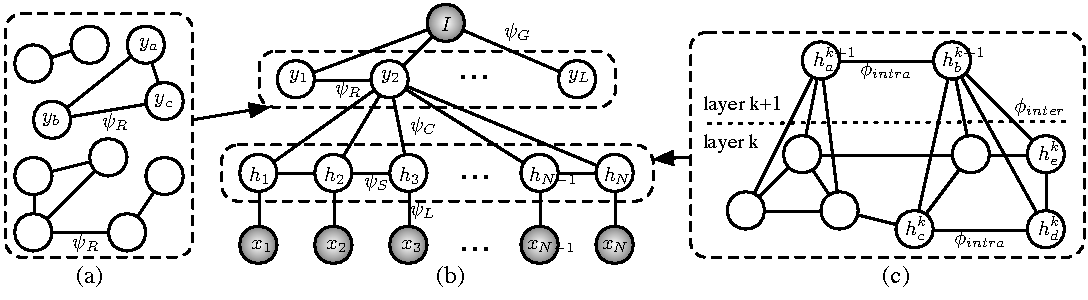
\includegraphics[width=0.95\linewidth]{graphmodel.pdf}
    \end{center}
    \caption{Example of a short caption, which should be centered.}
    \label{fig:graphmodel}
\end{figure*}

\subsection{Learning Parameters}
Due to the fact that pixel-level labels are not available during the training stage, we cannot use cross-validation \cite{kohli2009robust} to learn the weights for each potential. Inspired by \cite{vezhnevets2011weakly}, we scale the pairwise potentials and make them comparable to unary potentials instead of using cross-validation procedure.
After selecting the weights of each potential, we can learn the parameters of appearance model $\theta_a$ and topic model $\theta_t$ via an alternating optimization \cite{vezhnevets2011weakly}: 1) fix $\boldsymbol{h}$ and learn $\theta_a$, $\theta_t$; 2) fix $\theta_a$, $\theta_t$ and infer $\boldsymbol{h}$. The first step corresponds to a continues optimization problem, hence the optimal appearance parameters $\theta_a$ and topic parameters $\theta_t$ can be found efficiently via the existing supervised methods (\eg \cite{shotton2006textonboost}). The second step is a discrete optimization problem and we provide the details in Section \ref{sec:inference}.

\subsection{Joint Inference with Alternating Procedure}
\label{sec:inference}
Given an image $I$, our task is to assign each pixel a predefined semantic label. We achieve this as an energy minimization problem \eqref{eq:energyfunction}, in which our inference algorithm searches for optimal configuration of image-level label $\boldsymbol{y}^\star$ and superpixel-level label $\boldsymbol{h}^\star$. To efficiently minimize the energy function, we solve it in the following two alternating optimization steps:
\begin{equation}
    \label{eq:binaryCRF}
    \begin{aligned}
        \boldsymbol{y}^* = \arg\min_{\boldsymbol{y}} &\sum_{i} {\psi_{G}(y_i,I)} + \frac{1}{2} \psi_{C}(\boldsymbol{y},\boldsymbol{h}^*) \\ &+ \sum_{1 \le i,j \le L} {\psi_{R}(y_i,y_j)},
    \end{aligned}
\end{equation}
\begin{equation}
    \label{eq:multiclassCRF}
    \begin{aligned}
        \boldsymbol{h}^* = \arg\min_{\boldsymbol{h}} &\sum_{p} {\psi_{L}(h_p,x_p)} + \frac{1}{2} \psi_{C}(\boldsymbol{y}^*,\boldsymbol{h}) \\ &+ \sum_{(p,q) \in \mathcal{E}}{\psi_{S}(h_p,h_q)}.
    \end{aligned}
\end{equation}
As a standard binary CRF problem, the first subproblem in Equation \eqref{eq:binaryCRF} has an explicit solution which utilizes min-cut/max-flow algorithms (\eg the Dinic algorithm \cite{dinits1970algorithm}) to obtain the global optimal label configuration. And the second subproblem in Equation \eqref{eq:multiclassCRF} reduces to an energy minimization for a multi-class CRF. Although finding the global optimum for this energy function has been proved to be a NP-hard problem, there are various approximate methods for fast inference, such as approximate \textit{maximum a posteriori} (MAP) methods (\eg graph-cuts \cite{boykov2001fast}). In this paper, we adopt \textit{move making} approach \cite{boykov2001fast} that finds the optimal $\alpha$-expansion \cite{boykov2001fast,kolmogorov2004energy} by converting the problems into binary labeling  problems which can be solved efficiently using graph cuts techniques. The energy obtain by $\alpha$-expansion has been proved to be within a known factor of the global optimum \cite{boykov2001fast}. Considering the two alternate optimization steps together, we summarize our XXXX in Algorithm \ref{alg:energy}.


\renewcommand{\algorithmicrequire}{\textbf{Input:}}  % Use Input in the format of Algorithm
\renewcommand{\algorithmicensure}{\textbf{Output:}} % Use Output in the format of Algorithm

\begin{algorithm}
\caption{Energy minimization Inference}
\label{alg:energy}
\begin{algorithmic}[1]
    \Require
    a test image $I$ and its representation of superpixels $\{x_p\}$
    \Ensure
    the image-level label variables $\boldsymbol{y}$ and the superpixel-level label variables $\boldsymbol{h}$
    \State Construct the graphical model as shown in Figure \ref{fig:graphmodel}.
    \State Initialize $\boldsymbol{y}$ and $\boldsymbol{h}$ with the highest unary potential according to Equation \eqref{eq:global} and \eqref{eq:local}, respectively.
    \For{ iteration $t=1$ to $T$ }
        \State fix $\boldsymbol{y}$, optimize $\boldsymbol{h}$ via Equation \eqref{eq:multiclassCRF}
        \State fix $\boldsymbol{h}$, refine $\boldsymbol{y}$ via Equation \eqref{eq:binaryCRF}
    \EndFor
    \State Return the final configuration $\boldsymbol{y}$ and $\boldsymbol{h}$.
\end{algorithmic}
\end{algorithm}
